\documentclass[12pt,a4paper]{article}
% \documentclass[12pt,a4paper]{IEEEtran}

%\pdfoutput=1

\usepackage[utf8]{inputenc}
\usepackage[T1]{fontenc}
\usepackage[english]{babel}
\usepackage{amsmath}
\usepackage{amssymb}
\usepackage{mathabx}
\usepackage{lmodern}
\usepackage{units}
\usepackage{siunitx}
\usepackage{icomma}
\usepackage{graphicx}
\usepackage{caption}
\usepackage{subcaption}
\usepackage{color}
\usepackage{pgf}
\usepackage{listings}
\usepackage{color}

\definecolor{dkgreen}{rgb}{0,0.6,0}
\definecolor{gray}{rgb}{0.5,0.5,0.5}
\definecolor{mauve}{rgb}{0.58,0,0.82}

\lstset{frame=tb,
  language=Python,
  aboveskip=3mm,
  belowskip=3mm,
  showstringspaces=false,
  columns=flexible,
  basicstyle={\small\ttfamily},
  numbers=none,
  numberstyle=\tiny\color{gray},
  keywordstyle=\color{blue},
  commentstyle=\color{dkgreen},
  stringstyle=\color{mauve},
  breaklines=true,
  breakatwhitespace=true,
  tabsize=2
}

\usepackage[top=3cm,bottom=3cm,left=3cm,right=3cm]{geometry}
%\usepackage{times}
\newcommand{\N}{\ensuremath{\mathbbm{N}}}
\newcommand{\Z}{\ensuremath{\mathbbm{Z}}}
\newcommand{\Q}{\ensuremath{\mathbbm{Q}}}
\newcommand{\R}{\ensuremath{\mathbbm{R}}}
\newcommand{\C}{\ensuremath{\mathbbm{C}}}
\newcommand{\rd}{\ensuremath{\mathrm{d}}}
\newcommand{\id}{\ensuremath{\,\rd}}
\usepackage{hyperref}
% \usepackage{a4wide} % puts the page numbering further down the page.
\usepackage{pdfpages}
\usepackage{epstopdf}
\DeclareGraphicsExtensions{.eps}

\title{Locating the center of the Laurentide ice\\and tropospheric delay prediction\\using GNSS}
\author{Marcus Malmquist}
\date{\today}

\begin{document}
\pagenumbering{gobble}
% \maketitle
\noindent The raw data (output from GIPSY) for RESO can be seen in Figure~\ref{fig:reso} and more detailed data in Table~\ref{tab:reso}.
RESO was chosen is it was one of the stations that did not undergo an antenna change during 2005-2017 so there are no unnatural movements in the time-series.\\

\noindent It is evident that the radial error is a few times larger than the error in latitude and longitude.
The reason for this is that the radial position is more affected by error sources such as ionosphere, antenna phase center, satellite orbits and clocks.
The ionosphere and the satellite parameters have already been discussed but errors from the antenna phase center occur because the geometrical position of the antenna and the measured position are different.
This is because the measured center depends on frequency (so it will be different for L1 and L2) and the direction of the incomming signal.
\begin{table}[!ht]
  \centering
  \caption{The total move, average error and the average error relative to the total move}
  \begin{tabular}{|l|r|r|r|} \hline
    & Total move & Average error & Error/Move \\ \hline
    Longitude & \SI{-24.96}{\centi\meter} & \SI{1.18}{\milli\meter} & 0.47\% \\ \hline
    Latitude & \SI{-5.47}{\centi\meter} & \SI{0.11}{\milli\meter} & 0.20\% \\ \hline
    Radial & \SI{6.14}{\centi\meter} & \SI{4.06}{\milli\meter} & 6.61\% \\ \hline
    Longitude-Latitude & \SI{25.55}{\centi\meter} & \SI{1.19}{\milli\meter} & 0.47\% \\ \hline
    Longitude-Latitude-Radial & \SI{26.28}{\centi\meter} & \SI{4.23}{\milli\meter} & 1.61\% \\ \hline
  \end{tabular}
  \label{tab:reso}
\end{table}

\begin{figure}[!ht]
  \centering
  \noindent\makebox[\textwidth]{\scalebox{0.5}{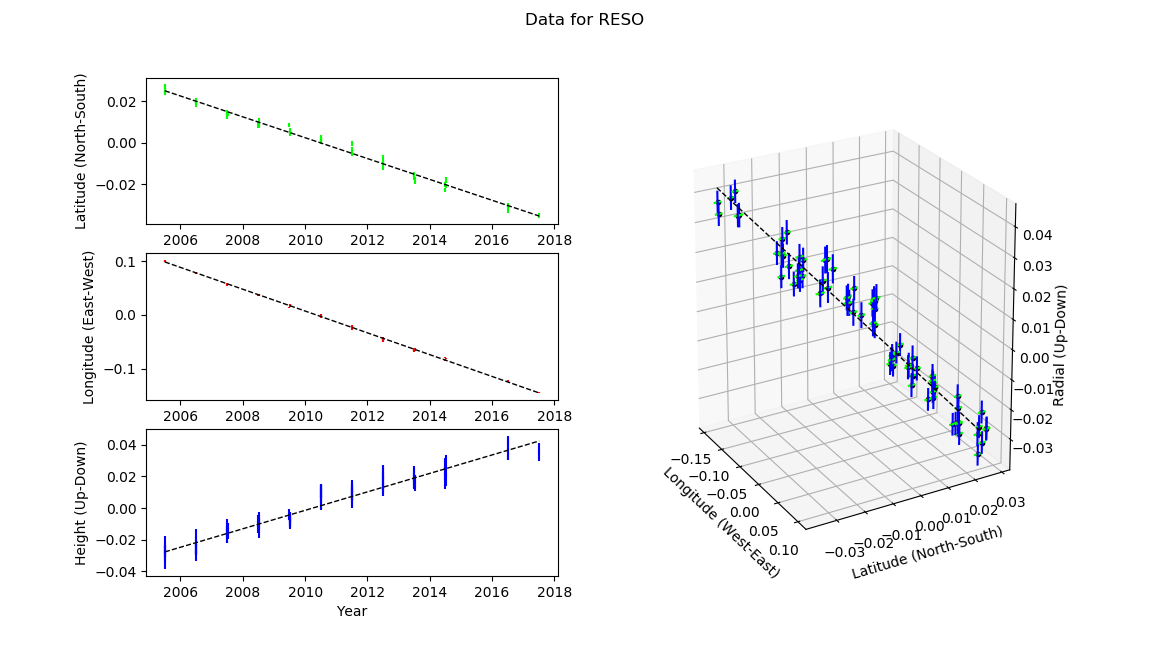
\includegraphics{task1/reso.png}}}
  \caption{The raw data plotted with error bars. Raw data means that no averaging or corrections (correcting for to antenna changes) have been made. It can be seen in the 3D plot that the radial error (blue) is a few times larger than the latitude and longitude error (green and red).}
  \label{fig:reso}
\end{figure}


\end{document}